\documentclass[aspectratio=169]{beamer}

\usetheme{Madrid}
\useinnertheme{circles}
\usecolortheme{default}

\usepackage[utf8]{inputenc}
\usepackage[T5]{fontenc}
\usepackage[vietnamese]{babel}
\usepackage{amsmath}
\usepackage{amssymb}
\usepackage{graphicx}
\usepackage{booktabs}
\usepackage{tikz}
\usetikzlibrary{arrows.meta, positioning}

\title[Cửa an ninh thông minh]{Cửa an ninh xác thực bằng khuôn mặt}
\subtitle{MVFNet $\cdot$ YOLOv11-Face $\cdot$ GFPGAN $\cdot$ Hiệu chỉnh hình học}
\author[ĐH Khoa học Tự nhiên]{Lưu Huy Minh Quang -- 23127016 \\ Hoàng Nhân -- 23127094 \\ Trần Cao Vân -- 23127141 \\ Nguyễn Trần Thiên Phú -- 23127246}
\institute[HCMUS]{Khoa Công nghệ Thông tin\\Đại học Khoa học Tự nhiên, ĐHQG TP.HCM\\[0.3em]\textit{Môn: Nhập môn lập trình điều khiển thiết bị thông minh}}
\date{Tháng 5, 2026}

\AtBeginSection[]{
  \begin{frame}[plain]
    \vfill
    \centering
      {\Large Phần \insertsectionnumber}\par\vspace{0.6em}
      \makebox[\textwidth][c]{%
      \begin{beamercolorbox}[wd=0.78\paperwidth,sep=12pt,center,rounded=true,shadow=true]{title}
        {\LARGE\bfseries \insertsectionhead}
      \end{beamercolorbox}
      }
    \vfill
  \end{frame}
}

\begin{document}

%------- TITLE -------
\begin{frame}
  \begin{center}
    \vspace{0.4em}
    \begin{beamercolorbox}[sep=8pt,center,shadow=true,rounded=true]{title}
      {\usebeamerfont{title}\inserttitle\par}
      \vspace{0.3em}
      {\usebeamerfont{subtitle}\insertsubtitle\par}
    \end{beamercolorbox}

    \vspace{0.8em}
    \begin{block}{\centering Nhóm thực hiện}
      \centering
      \begin{tabular}{ll}
        Lưu Huy Minh Quang & 23127016 \\
        Hoàng Nhân & 23127094 \\
        Trần Cao Vân & 23127141 \\
        Nguyễn Trần Thiên Phú & 23127246 \\
      \end{tabular}\\[0.5em]
      \textit{Khoa CNTT -- ĐH Khoa học Tự nhiên, ĐHQG TP.HCM}\\
      \textit{Môn: Nhập môn lập trình điều khiển thiết bị thông minh}
    \end{block}

    \vspace{0.5em}
    {\large \insertdate}
  \end{center}
\end{frame}

%------- MỤC LỤC -------
\begin{frame}{Nội dung trình bày}
  \vspace{0.4em}
  \begin{enumerate}
    \item Bài toán, phạm vi và bối cảnh
    \item Lý do chọn công nghệ
    \item Kiến trúc hệ thống và vòng lặp điều khiển
    \item Pipeline AI tái tạo khuôn mặt 3D
    \item Rủi ro, thách thức và hướng giải quyết
    \item Dataset và cách đánh giá
    \item Mockup sản phẩm và giao diện
  \end{enumerate}
\end{frame}

%============================
\section{Bài toán, phạm vi và bối cảnh}
%============================

\begin{frame}{Giới thiệu đề tài}
  \begin{block}{Sản phẩm đề xuất}
    \textbf{Cửa an ninh thông minh} -- xác thực danh tính người dùng bằng khuôn mặt 3D, tự động mở/khóa cửa thông qua hệ thống thiết bị thông minh.
  \end{block}

  \vspace{0.4em}
  \textbf{Ý tưởng cốt lõi:}
  \begin{itemize}
    \item Camera IoT gắn tại cửa thu ảnh khuôn mặt người đứng trước
    \item Hệ thống AI phía server \textbf{tái tạo mô hình 3D} từ ảnh 2D
    \item So khớp mô hình 3D với cơ sở dữ liệu danh tính đã đăng ký
    \item Nếu khớp $\to$ gửi tín hiệu mở cửa; nếu không $\to$ từ chối + cảnh báo
  \end{itemize}

  \vspace{0.4em}
  \begin{alertblock}{Tại sao dùng 3D thay vì 2D?}
    Xác thực 2D dễ bị đánh lừa bởi ảnh in, video phát lại hoặc màn hình. Tái tạo mesh 3D buộc hệ thống phải hiểu \textbf{cấu trúc hình học} khuôn mặt -- khó giả mạo hơn nhiều.
  \end{alertblock}
\end{frame}

\begin{frame}{Lý do chọn đề tài}
  \begin{columns}[T]
    \column{0.48\textwidth}
      \begin{block}{Góc nhìn học thuật}
        \begin{itemize}
          \item Kết hợp 3 lĩnh vực: \textbf{Computer Vision}, \textbf{AI} và \textbf{IoT} trong một pipeline khép kín
          \item Thể hiện rõ tư duy \textit{điều khiển thiết bị thông minh}: cảm nhận $\to$ xử lý $\to$ hành động $\to$ phản hồi
          \item Bài toán có độ khó vừa phải, phù hợp đồ án môn học
        \end{itemize}
      \end{block}

    \column{0.48\textwidth}
      \begin{block}{Góc nhìn ứng dụng}
        \begin{itemize}
          \item Nhà thông minh (smart home)
          \item Văn phòng, phòng server, phòng lab
          \item Chung cư, ký túc xá
          \item Kiosk tự phục vụ (ngân hàng, sân bay)
          \item Có thể mở rộng: chấm công, điểm danh
        \end{itemize}
      \end{block}
  \end{columns}
\end{frame}

\begin{frame}[t]{Mô tả bài toán}
  \footnotesize
  \textbf{Mục tiêu bài toán và phạm vi}
  \begin{itemize}\setlength{\itemsep}{0pt}
    \item \textbf{Mục tiêu:} Xác thực khuôn mặt người đứng trước cửa, trả về \texttt{PASS}/\texttt{DENY} và điều khiển relay.
    \item \textbf{Phạm vi:} ESP32-CAM chụp ảnh 2D; server xử lý AI; dashboard đăng ký khuôn mặt và xem log.
    \item \textbf{Giới hạn:} ảnh ESP32-CAM có thể độ phân giải thấp, mờ, nhiễu hoặc thiếu sáng.
  \end{itemize}

  \vspace{0.2em}
  \textbf{Đầu vào (Input)}
  \begin{itemize}\setlength{\itemsep}{0pt}
    \item Ảnh khuôn mặt 2D từ ESP32-CAM hoặc IP camera.
    \item Có thể nhiều người, góc nghiêng, khuôn mặt nhỏ hoặc che khuất.
  \end{itemize}

  \vspace{0.2em}
  \textbf{Ràng buộc kỹ thuật}
  \begin{itemize}\setlength{\itemsep}{0pt}
    \item Chỉ có 1 ảnh 2D nên thiếu thông tin chiều sâu.
    \item ESP32-CAM giới hạn RAM, CPU và băng thông nên không huấn luyện/tinh chỉnh model trực tiếp trên thiết bị.
    \item Laptop/server dùng để chạy model, xuất tham số/cấu hình cần thiết rồi nạp xuống thiết bị; dữ liệu sinh trắc cần bảo mật.
  \end{itemize}

  \vspace{0.2em}
  \textbf{Đầu ra (Output)}
  \begin{itemize}\setlength{\itemsep}{0pt}
    \item Mesh 3D + texture khuôn mặt; kết quả \texttt{PASS}/\texttt{DENY}; lệnh relay; log ra/vào.
  \end{itemize}
\end{frame}

%============================
\section{Lý do chọn công nghệ}
%============================

\begin{frame}{Lý do chọn công nghệ}
  \footnotesize
  \begin{columns}[T]
    \column{0.48\textwidth}
      \textbf{YOLOv11-Face -- phát hiện khuôn mặt}
      \begin{itemize}\setlength{\itemsep}{0.2em}
        \item Phù hợp bước đầu pipeline: tìm mặt nhanh trong ảnh ESP32-CAM.
        \item Hỗ trợ nhiều khuôn mặt trong một frame, dễ crop vùng cần xử lý.
      \end{itemize}

      \vspace{0.35em}
      \textbf{GFPGAN -- tăng cường ảnh đầu vào}
      \begin{itemize}\setlength{\itemsep}{0.2em}
        \item ESP32-CAM có thể cho ảnh mờ, nhiễu, thiếu sáng hoặc độ phân giải thấp.
        \item GFPGAN giúp phục hồi chi tiết mặt trước khi tái tạo 3D.
      \end{itemize}

    \column{0.48\textwidth}
      \textbf{MVFNet + 3DMM -- lõi tái tạo 3D}
      \begin{itemize}\setlength{\itemsep}{0.2em}
        \item Tạo mesh 3D và tham số nhận dạng từ ảnh khuôn mặt 2D.
        \item Vector identity $\alpha_{\text{id}}$ có thể dùng để so khớp danh tính.
      \end{itemize}

      \vspace{0.35em}
      \textbf{Hậu xử lý và matching}
      \begin{itemize}\setlength{\itemsep}{0.2em}
        \item Laplacian smoothing giảm nhiễu hình học trên mesh.
        \item Matching theo ngưỡng $\theta$ giúp chuyển kết quả AI thành \texttt{PASS}/\texttt{DENY}.
      \end{itemize}
  \end{columns}

  \vspace{0.8em}
  \textbf{Tóm lại:}
  ESP32-CAM chỉ thu ảnh và điều khiển relay; phần AI nặng chạy trên laptop/server.
\end{frame}

%============================
\section{Kiến trúc hệ thống và vòng lặp điều khiển}
%============================

\begin{frame}{Vòng lặp điều khiển thiết bị thông minh}
  \vspace{0.2em}
  \begin{center}
  \begin{tikzpicture}[
    stagebox/.style={rectangle, rounded corners=3pt, draw=blue!70, fill=blue!7,
      text width=3.65cm, align=left, font=\scriptsize, inner sep=5pt,
      minimum height=1.15cm},
    sense/.style={stagebox, draw=teal!70!black, fill=teal!8},
    ai/.style={stagebox, draw=blue!70, fill=blue!7},
    decision/.style={stagebox, draw=orange!80!black, fill=orange!10},
    action/.style={stagebox, draw=green!55!black, fill=green!9},
    arr/.style={-{Stealth[length=2mm]}, thick, blue!70},
    fb/.style={-{Stealth[length=2mm]}, thick, red!65}
  ]
    \node[sense] (sense) {
      \textbf{1. Cảm nhận}\\
      ESP32-CAM chụp ảnh người đứng trước cửa và gửi về server.
    };
    \node[ai, right=0.55cm of sense] (perceive) {
      \textbf{2. Nhận thức}\\
      YOLOv11-Face phát hiện khuôn mặt và kiểm tra chất lượng ảnh.
    };
    \node[ai, right=0.55cm of perceive] (process) {
      \textbf{3. Xử lý}\\
      GFPGAN tăng cường ảnh, MVFNet tái tạo mesh 3D.
    };
    \node[decision, below=0.9cm of process] (eval) {
      \textbf{4. Ra quyết định}\\
      So khớp đặc trưng 3D với database và ngưỡng xác thực.
    };
    \node[action, left=0.55cm of eval] (act) {
      \textbf{5. Hành động}\\
      Mở relay nếu \texttt{PASS}; từ chối và ghi log nếu \texttt{DENY}.
    };

    \draw[arr] (sense.east) -- (perceive.west);
    \draw[arr] (perceive.east) -- (process.west);
    \draw[arr] (process.south) -- (eval.north);
    \draw[arr] (eval.west) -- (act.east);
    \draw[fb] (act.west) to[out=180, in=-90]
      node[midway, left, align=right, font=\scriptsize, red!70!black]
      {Feedback: ảnh kém\\$\to$ chụp lại / enhance} (sense.south);
  \end{tikzpicture}
  \end{center}

  \vspace{0.3em}
  \begin{alertblock}{Điểm điều khiển chính}
    \small
    Hệ thống tạo vòng lặp kín: cảm biến thu ảnh $\to$ AI xử lý và ra quyết định $\to$ thiết bị thực thi $\to$ phản hồi khi ảnh đầu vào chưa đạt chất lượng.
  \end{alertblock}
\end{frame}

\subsection{Kiến trúc hệ thống}

\begin{frame}{Kiến trúc tổng thể -- 3 lớp}
  \begin{center}
  \begin{tikzpicture}[
    layerbox/.style={rectangle, rounded corners=4pt, text width=3.45cm,
      align=center, minimum height=1.55cm, font=\small\bfseries, inner sep=6pt},
    iotbox/.style={layerbox, draw=teal!70!black, fill=teal!9},
    aibox/.style={layerbox, draw=blue!70, fill=blue!8},
    appbox/.style={layerbox, draw=orange!80!black, fill=orange!10},
    arr/.style={-{Stealth[length=2mm]}, thick, blue!70}
  ]
    \node[iotbox] (iot) {Lớp IoT\\{\scriptsize Thu ảnh, điều khiển relay}};
    \node[aibox, right=0.9cm of iot] (ai) {Lớp AI\\{\scriptsize Phát hiện, tái tạo 3D, xác thực}};
    \node[appbox, right=0.9cm of ai] (app) {Lớp Ứng dụng\\{\scriptsize Đăng ký, quản lý, giám sát}};

    \draw[arr] (iot) -- node[above, font=\scriptsize]{ảnh 2D} (ai);
    \draw[arr] (ai) -- node[above, font=\scriptsize]{log / kết quả} (app);
    \draw[arr] (ai.south) to[out=-100,in=-80,looseness=1.2]
      node[below, font=\scriptsize]{PASS/DENY + lệnh relay} (iot.south);
  \end{tikzpicture}
  \end{center}

  \vspace{0.6em}
  \begin{block}{Cách phân chia trách nhiệm}
    \small
    ESP32-CAM không dùng để huấn luyện hoặc chỉnh sửa model trực tiếp. Laptop/server đảm nhiệm phần xử lý nặng và xuất tham số/cấu hình triển khai; thiết bị chỉ nạp các tham số cần thiết, chạy phần nhẹ và thực thi lệnh mở/khóa cửa.
  \end{block}
\end{frame}

\begin{frame}{Lớp IoT -- Edge / Thiết bị}
  \begin{columns}[T]
    \column{0.48\textwidth}
      \begin{block}{Phần cứng}
        \begin{itemize}
          \item \textbf{ESP32-CAM}: camera nhúng giá rẻ, Wi-Fi tích hợp
          \item \textbf{Relay module}: điều khiển khóa điện từ
          \item \textbf{LCD/LED}: hiển thị trạng thái xanh/đỏ
          \item \textbf{Buzzer}: cảnh báo âm thanh
        \end{itemize}
      \end{block}

    \column{0.48\textwidth}
      \begin{block}{Nhiệm vụ}
        \begin{itemize}
          \item Chụp ảnh khuôn mặt trước cửa
          \item Gửi ảnh JPEG và metadata về server
          \item Nạp tham số/cấu hình đã xuất từ laptop/server
          \item Nhận kết quả \texttt{PASS}/\texttt{DENY}
          \item Bật/tắt relay theo lệnh phản hồi
        \end{itemize}
      \end{block}
  \end{columns}

  \vspace{0.4em}
  \begin{alertblock}{Giới hạn cần lưu ý}
    \small
    ESP32-CAM có RAM, CPU và chất lượng ảnh hạn chế, nên không train/tune trên phần cứng. Model được chạy và tinh chỉnh trên laptop/server; thiết bị chỉ nhận tham số hoặc cấu hình triển khai.
  \end{alertblock}
\end{frame}

\begin{frame}{Lớp AI -- Laptop/Server xử lý}
  \begin{block}{Pipeline xử lý chính}
    \begin{enumerate}
      \item \textbf{Chuẩn bị model}: chạy thử, huấn luyện/tinh chỉnh và xuất weight, threshold hoặc cấu hình triển khai trên laptop/server.
      \item \textbf{YOLOv11-Face}: phát hiện khuôn mặt và crop vùng cần xử lý.
      \item \textbf{GFPGAN}: tăng cường chất lượng ảnh mờ, nhiễu hoặc thiếu sáng.
      \item \textbf{MVFNet + 3DMM}: tái tạo mesh 3D từ ảnh khuôn mặt 2D.
      \item \textbf{Laplacian Smoothing}: làm mịn mesh, giảm nhiễu hình học.
      \item \textbf{Matching Engine}: so khớp đặc trưng 3D với database đã đăng ký.
    \end{enumerate}
  \end{block}

  \vspace{0.3em}
  \begin{alertblock}{Kết quả trả về}
    \small
    Laptop/server trả về kết quả xác thực \texttt{PASS}/\texttt{DENY}, độ tin cậy, lệnh điều khiển relay và các tham số/cấu hình cần nạp xuống thiết bị.
  \end{alertblock}
\end{frame}

\begin{frame}{Lớp Ứng dụng -- Web / Dashboard}
  \begin{columns}[T]
    \column{0.48\textwidth}
      \begin{block}{Chức năng vận hành}
        \begin{itemize}
          \item Đăng ký khuôn mặt mới
          \item Quản lý danh sách user được phép vào
          \item Cấu hình ngưỡng xác thực
          \item Theo dõi trạng thái thiết bị
        \end{itemize}
      \end{block}

    \column{0.48\textwidth}
      \begin{block}{Giám sát và nhật ký}
        \begin{itemize}
          \item Xem nhật ký ra/vào theo thời gian
          \item Lưu ảnh, kết quả xác thực và confidence
          \item Cảnh báo truy cập bị từ chối
          \item Hỗ trợ kiểm tra lại các sự kiện bất thường
        \end{itemize}
      \end{block}
  \end{columns}
\end{frame}

\begin{frame}{Luồng dữ liệu giữa các lớp}
  \begin{center}
  \begin{tikzpicture}[
    layer/.style={rectangle, rounded corners, text width=3cm, align=center, minimum height=1cm, font=\small\bfseries},
    layer teal/.style={layer, draw=teal, fill=teal!10},
    layer blue/.style={layer, draw=blue, fill=blue!10},
    layer orange/.style={layer, draw=orange, fill=orange!10},
    data/.style={-{Stealth}, thick, font=\scriptsize}
  ]
    \node[layer teal] (iot) {Lớp IoT\\{\scriptsize ESP32-CAM}};
    \node[layer blue, right=2.5cm of iot] (ai) {Lớp AI\\{\scriptsize Server/GPU}};
    \node[layer orange, right=2.5cm of ai] (app) {Lớp Ứng dụng\\{\scriptsize Web Dashboard}};

    \draw[data, teal] (iot.north east) -- node[above]{ảnh 2D (JPEG)} (ai.north west);
    \draw[data, blue] (ai.south west) -- node[below]{PASS/DENY + relay cmd} (iot.south east);
    \draw[data, orange] (ai.north east) -- node[above]{log, mesh 3D} (app.north west);
    \draw[data, orange!70!red] (app.south west) -- node[below]{config, user DB} (ai.south east);
  \end{tikzpicture}
  \end{center}

  \vspace{0.5em}
  \begin{columns}[T]
    \column{0.48\textwidth}
      \textbf{IoT $\to$ AI:}
      \begin{itemize}
        \item ESP32-CAM chụp ảnh JPEG, gửi qua HTTP POST
        \item Kèm metadata: device\_id, timestamp
      \end{itemize}
    \column{0.48\textwidth}
      \textbf{AI $\to$ IoT:}
      \begin{itemize}
        \item Response JSON: \texttt{\{result, confidence, cmd\}}
        \item ESP32 nhận lệnh $\to$ bật/tắt relay
      \end{itemize}
  \end{columns}
\end{frame}

%============================
\section{Pipeline AI tái tạo khuôn mặt 3D}
%============================

\begin{frame}{Pipeline xử lý AI -- Tổng quan}
  \textbf{Quy trình 5 bước}

  \vspace{0.2em}
  \begin{center}
    \footnotesize
    \texttt{Ảnh 2D}
    $\xrightarrow{\text{\textbf{1.} YOLOv11}}$ \texttt{Crop mặt}
    $\xrightarrow{\text{\textbf{2.} GFPGAN}}$ \texttt{Ảnh nét}
    $\xrightarrow{\text{\textbf{3.} MVFNet}}$ \texttt{Mesh 3D thô}
    $\xrightarrow{\text{\textbf{4.} Smooth}}$ \texttt{Mesh mịn}
    $\xrightarrow{\text{\textbf{5.} Match}}$ \texttt{Kết quả}
  \end{center}

  \vspace{0.4em}
  \begin{columns}[T]
    \column{0.48\textwidth}
      \textbf{Bước 1: YOLOv11-Face}
      \begin{itemize}
        \item Phát hiện bounding box khuôn mặt
        \item Crop với hệ số mở rộng $s = 1.2$:
          \[ \text{Size} = \max(w, h) \times 1.2 \]
        \item Dịch tâm xuống $0.14 \times$ Size (bao phủ cằm)
        \item Xử lý được nhiều mặt trong 1 frame
      \end{itemize}

    \column{0.48\textwidth}
      \textbf{Bước 2: GFPGAN (Image Enhancement)}
      \begin{itemize}
        \item Phục hồi ảnh mờ, nhiễu, độ phân giải thấp
        \item Sử dụng GAN với \textit{generative facial prior}
        \item Tái tạo chi tiết vùng mắt, mũi, môi
        \item Đảm bảo ảnh đầu vào cho MVFNet luôn đạt chất lượng tối ưu
      \end{itemize}
  \end{columns}
\end{frame}

\begin{frame}{Pipeline xử lý AI -- Tái tạo 3D}
  \textbf{Bước 3: MVFNet + 3DMM -- Hồi quy khuôn mặt 3D}

  \vspace{0.3em}
  Mô hình hóa khuôn mặt bằng \textbf{3D Morphable Model}:
  \[
    S = \bar{S} + B_{\text{id}}\,\alpha_{\text{id}} + B_{\text{exp}}\,\alpha_{\text{exp}}
  \]
  \begin{itemize}
    \item $\bar{S}$: hình dạng khuôn mặt trung bình (mean face)
    \item $B_{\text{id}} \in \mathbb{R}^{3N \times 199}$: cơ sở hình dạng nhận dạng (PCA)
    \item $B_{\text{exp}} \in \mathbb{R}^{3N \times 29}$: cơ sở biểu cảm
    \item $\alpha_{\text{id}}, \alpha_{\text{exp}}$: tham số cá nhân -- \textbf{đây là vector dùng để xác thực}
  \end{itemize}
  Mạng VggEncoder trích xuất vector 257 chiều (identity + expression + pose) từ ảnh 2D.
\end{frame}

\begin{frame}{Pipeline xử lý AI -- Hậu xử lý mesh}
  \textbf{Bước 4: Laplacian Smoothing}

  \vspace{0.4em}
  Hiệu chỉnh tọa độ đỉnh mesh theo trung bình lân cận:
  \[
    L(v_i) = \frac{1}{|N(i)|} \sum_{j \in N(i)} (v_j - v_i)
  \]

  \vspace{0.2em}
  \begin{itemize}
    \item Loại bỏ nhiễu răng cưa trên bề mặt mesh sau khi tái tạo.
    \item Làm mượt các vùng bị méo do ảnh đầu vào mờ, nhiễu hoặc thiếu sáng.
    \item Giữ nguyên cấu trúc tổng thể khuôn mặt, tránh làm mất đặc trưng nhận dạng.
    \item Mesh mịn hơn giúp bước so khớp 3D ổn định và chính xác hơn.
  \end{itemize}
\end{frame}

\begin{frame}{Pipeline xử lý AI -- Texture \& Xác thực}
  \begin{columns}[T]
    \column{0.48\textwidth}
      \textbf{Bước 4b: Texture Fusion}

      \vspace{0.2em}
      Hòa trộn màu sắc đa góc nhìn:
      \[
        w = \max(0,\; \vec{n} \cdot \vec{v})
      \]
      \begin{itemize}
        \item $\vec{n}$: pháp tuyến đỉnh mesh
        \item $\vec{v}$: hướng camera
        \item Chọn màu từ góc nhìn tốt nhất
        \item Giảm vùng texture bị kéo giãn hoặc thiếu chi tiết
      \end{itemize}

    \column{0.48\textwidth}
      \textbf{Bước 5: Xác thực danh tính}

      \vspace{0.2em}
      So sánh $\alpha_{\text{id}}$ với database:
      \[
        \text{sim}(\alpha_{\text{id}}^{\text{input}},\; \alpha_{\text{id}}^{\text{DB}}) \geq \theta
      \]
      \begin{itemize}
        \item Nếu đạt ngưỡng: \texttt{PASS} $\to$ gửi lệnh mở relay.
        \item Nếu không đạt: \texttt{DENY} $\to$ từ chối và ghi log.
        \item Threshold $\theta$ được tinh chỉnh trên laptop/server trước khi triển khai.
      \end{itemize}
  \end{columns}
\end{frame}

%============================
\section{Rủi ro, thách thức và hướng giải quyết}
%============================

\begin{frame}{Rủi ro / thách thức và hướng giải quyết}
  \footnotesize
  \begin{columns}[T]
    \column{0.48\textwidth}
      \textbf{Chất lượng ảnh ESP32-CAM}
      \begin{itemize}\setlength{\itemsep}{0.15em}
        \item Ảnh ban đêm yếu sáng, mờ, nhiễu hoặc ngược sáng.
        \item Khuôn mặt nhỏ, lệch góc, bị che bởi khẩu trang/nón.
        \item \textbf{Xử lý:} thêm LED/IR, kiểm tra chất lượng ảnh, chụp lại nhiều frame, crop đúng mặt và dùng GFPGAN trước MVFNet.
      \end{itemize}

      \vspace{0.25em}
      \textbf{Độ trễ hệ thống}
      \begin{itemize}\setlength{\itemsep}{0.15em}
        \item Latency mạng khi ESP32-CAM gửi ảnh JPEG lên server.
        \item AI inference có thể vượt mục tiêu phản hồi nhanh.
        \item \textbf{Xử lý:} giảm kích thước ảnh gửi, timeout rõ ràng, cache model trên server, log thời gian từng bước.
      \end{itemize}

    \column{0.48\textwidth}
      \textbf{Sai nhận dạng}
      \begin{itemize}\setlength{\itemsep}{0.15em}
        \item False positive: mở cửa cho người không hợp lệ.
        \item False negative: từ chối người hợp lệ khi ảnh xấu.
        \item \textbf{Xử lý:} tinh chỉnh ngưỡng $\theta$, yêu cầu chụp lại khi confidence thấp, lưu ảnh sự kiện để kiểm tra sau.
      \end{itemize}

      \vspace{0.25em}
      \textbf{Bảo mật và vận hành}
      \begin{itemize}\setlength{\itemsep}{0.15em}
        \item Dữ liệu khuôn mặt là dữ liệu sinh trắc nhạy cảm.
        \item Thiết bị IoT có thể mất kết nối hoặc bị gọi API giả.
        \item \textbf{Xử lý:} xác thực device\_id/token, giới hạn quyền dashboard, mã hóa dữ liệu nhạy cảm và có chế độ fail-safe.
      \end{itemize}
  \end{columns}
\end{frame}

%============================
\section{Dataset và cách đánh giá}
%============================

\begin{frame}{Dataset kiểm thử}
  \footnotesize
  \begin{columns}[T]
    \column{0.48\textwidth}
      \textbf{Dataset công khai}
      \begin{itemize}\setlength{\itemsep}{0.25em}
        \item \textbf{AFLW2000-3D} \cite{aflw}: ảnh khuôn mặt có pose lớn và annotation 3D.
        \item Dùng để kiểm tra detect/crop, pose khó và độ ổn định tái tạo 3D.
        \item Phù hợp đánh giá phần AI trước khi gắn với phần cứng thật.
      \end{itemize}

      \vspace{0.35em}
      \textbf{Dataset tự chụp}
      \begin{itemize}\setlength{\itemsep}{0.25em}
        \item Chụp bằng ESP32-CAM trong đúng bối cảnh cửa ra/vào.
        \item Mỗi người: chính diện, nghiêng trái/phải, xa/gần, sáng/yếu sáng.
        \item Thêm mẫu không hợp lệ để đo khả năng từ chối người lạ.
      \end{itemize}

    \column{0.48\textwidth}
      \textbf{Chia tập thử nghiệm}
      \begin{itemize}\setlength{\itemsep}{0.25em}
        \item \textbf{Enroll set}: ảnh đăng ký khuôn mặt hợp lệ.
        \item \textbf{Test same-user}: ảnh cùng người nhưng khác góc/ánh sáng.
        \item \textbf{Test unknown}: ảnh người không có trong database.
      \end{itemize}

      \vspace{0.35em}
      \textbf{Kịch bản kiểm thử}
      \begin{itemize}\setlength{\itemsep}{0.25em}
        \item Kiểm thử offline trên laptop/server trước.
        \item Sau đó kiểm thử end-to-end: ESP32-CAM $\to$ server $\to$ relay/log.
        \item Ghi lại ảnh, kết quả, confidence và thời gian xử lý.
      \end{itemize}
  \end{columns}
\end{frame}

\begin{frame}{Chỉ số đánh giá}
  \footnotesize
  \begin{columns}[T]
    \column{0.5\textwidth}
      \textbf{Xác thực danh tính}
      \begin{itemize}\setlength{\itemsep}{0.2em}
        \item \textbf{Accuracy}: tỷ lệ quyết định đúng trên toàn bộ lượt thử.
        \item \textbf{FAR}: tỷ lệ người lạ bị nhận nhầm là hợp lệ.
        \item \textbf{FRR}: tỷ lệ người hợp lệ bị từ chối.
        \item Ma trận nhầm lẫn: \texttt{PASS}/\texttt{DENY} so với nhãn thật.
      \end{itemize}

      \vspace{0.25em}
      \[
        \text{FAR} = \frac{\text{False Accept}}{\text{Unknown Attempts}},
        \quad
        \text{FRR} = \frac{\text{False Reject}}{\text{Valid Attempts}}
      \]

    \column{0.46\textwidth}
      \textbf{Chất lượng pipeline}
      \begin{itemize}\setlength{\itemsep}{0.2em}
        \item Tỷ lệ phát hiện được mặt trong frame.
        \item Tỷ lệ ảnh phải chụp lại hoặc enhance.
        \item Similarity score trung bình theo từng điều kiện ánh sáng/góc nhìn.
      \end{itemize}

      \vspace{0.25em}
      \textbf{Hiệu năng hệ thống}
      \begin{itemize}\setlength{\itemsep}{0.2em}
        \item Tổng latency: chụp ảnh + gửi mạng + inference + trả lệnh.
        \item Mục tiêu phản hồi: dưới 3 giây trong điều kiện mạng ổn định.
        \item Tỷ lệ lỗi kết nối và số lần timeout.
      \end{itemize}
  \end{columns}
\end{frame}

%============================
\section{Mockup sản phẩm và giao diện}
%============================

\begin{frame}{Mockup sản phẩm -- Cửa an ninh}
  \begin{columns}[T]
    \column{0.62\textwidth}
      \begin{center}
        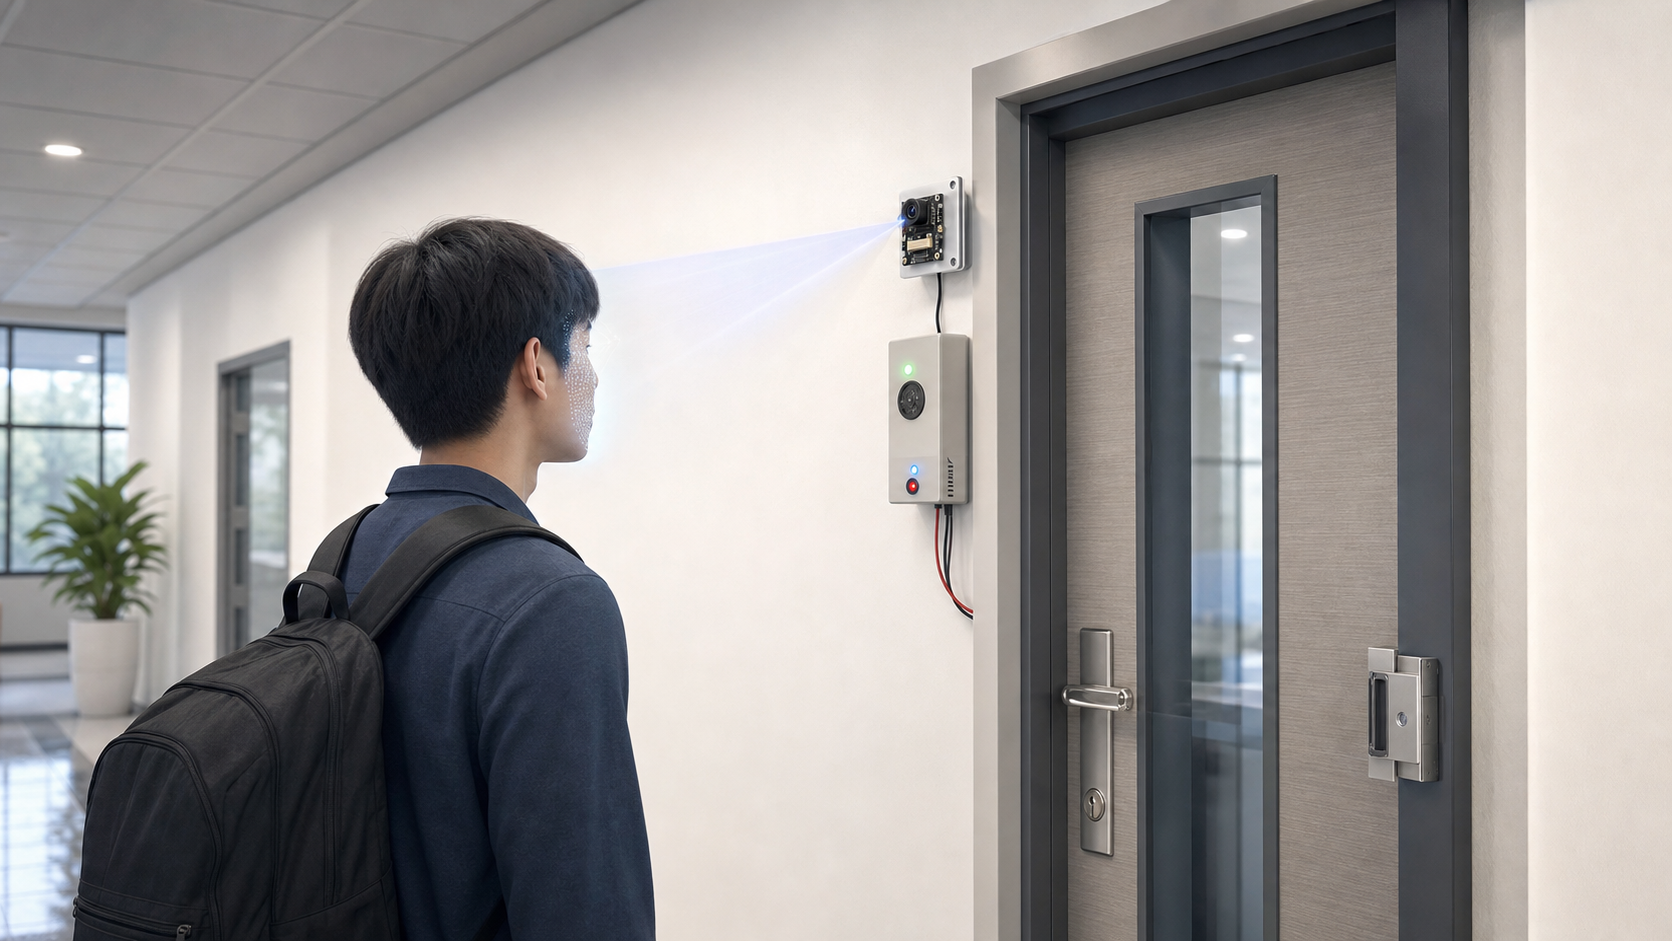
\includegraphics[width=\linewidth,height=0.72\textheight,keepaspectratio]{images/smart_door_mockup.png}
      \end{center}

    \column{0.34\textwidth}
      \footnotesize
      \textbf{Bố trí phần cứng tại cửa}
      \begin{itemize}\setlength{\itemsep}{0.18em}
        \item ESP32-CAM đặt ngang tầm mặt, chụp ảnh người đứng trước cửa.
        \item Relay nối khóa điện từ, chỉ mở khi server trả \texttt{PASS}.
        \item LED/buzzer báo trạng thái xử lý, cho phép vào hoặc từ chối.
      \end{itemize}

      \vspace{0.2em}
      \textbf{Luồng triển khai}
      \begin{itemize}\setlength{\itemsep}{0.18em}
        \item AI chạy trên laptop/server để tránh quá tải phần cứng.
        \item ESP32-CAM chỉ gửi ảnh, nhận lệnh và điều khiển relay.
      \end{itemize}
  \end{columns}
\end{frame}

\begin{frame}{Mockup giao diện Web Dashboard}
  \begin{center}
    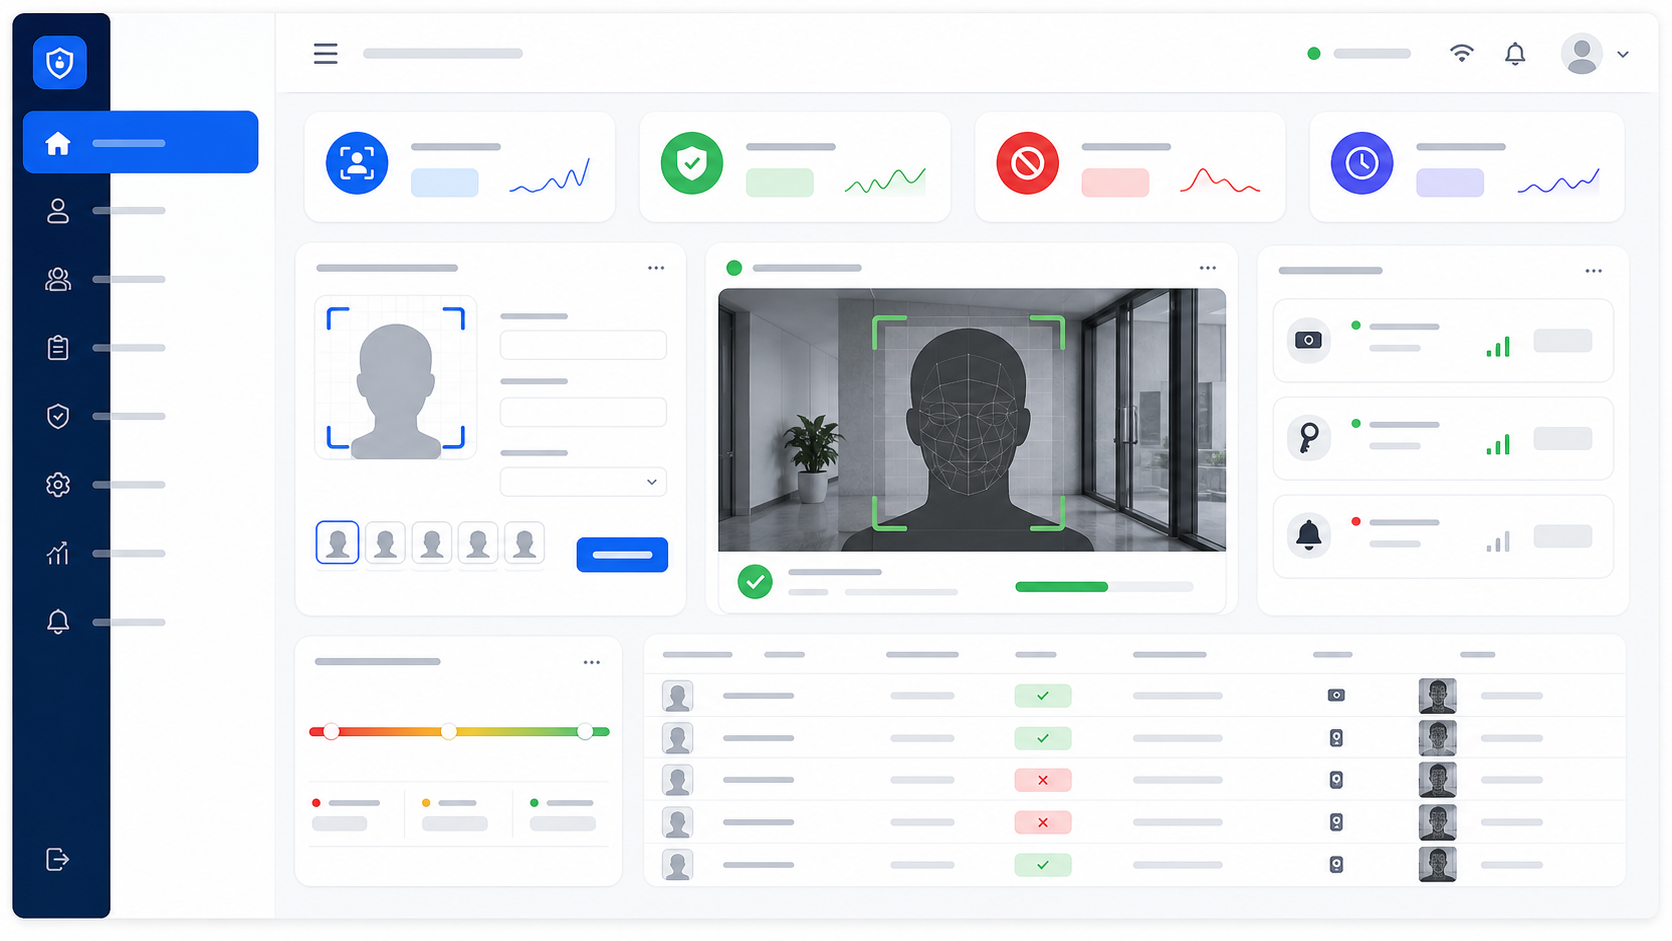
\includegraphics[width=0.95\textwidth,height=0.78\textheight,keepaspectratio]{images/dashboard_mockup.png}
  \end{center}
\end{frame}

%------- TÀI LIỆU THAM KHẢO -------
\begin{frame}{Tài liệu tham khảo}
  \footnotesize
  \begin{thebibliography}{99}
    \bibitem{mvfnet} F. Wu \textit{et al.}, ``MVFNet: Multi-View 3D Face Morphable Model Regression,'' \textit{CVPR}, 2019.
    \bibitem{yolo} Ultralytics, ``YOLOv11,'' GitHub, 2024.
    \bibitem{gfpgan} X. Wang \textit{et al.}, ``GFPGAN: Towards Real-World Blind Face Restoration with Generative Facial Prior,'' \textit{CVPR}, 2021.
    \bibitem{3dmm} V. Blanz \& T. Vetter, ``A Morphable Model for the Synthesis of 3D Faces,'' \textit{SIGGRAPH}, 1999.
    \bibitem{lap} D. A. Field, ``Laplacian smoothing and Delaunay triangulations,'' \textit{Comm. in Applied Numerical Methods}, 1988.
    \bibitem{aflw} X. Zhu \textit{et al.}, ``Face Alignment Across Large Poses: A 3D Solution,'' \textit{CVPR}, 2016.
  \end{thebibliography}
\end{frame}

%------- CLOSING -------
\begin{frame}[plain]
  \begin{center}
    \vspace{2.5cm}
    {\Huge \textbf{Cảm ơn!}}\\[0.8em]
    {\Large Câu hỏi \& Thảo luận}
  \end{center}
\end{frame}

\end{document}
